\documentclass{jsarticle}

\usepackage[dvipdfmx]{graphicx}

\begin{document}

\title{情報工学5 HW01}
\author{08-132021 堀江慧}
\date{}
\maketitle{}

\begin{abstract}
\begin{center}
第1回課題 OpenCVの使い方
\end{center}
\end{abstract}

\section{例題プログラムの実行}

\subsection{grayscale.cc}

\subsubsection{source code}
\begin{verbatim}
     1	#include<iostream>
     2	#include<opencv2/core/core.hpp>
     3	#include<opencv2/imgproc/imgproc.hpp>
     4	#include<opencv2/highgui/highgui.hpp>
     5	
     6	using namespace cv;
     7	using namespace std;
     8	
     9	int main(int argc, char*argv[]){
    10	  if (argc <= 1){
    11	    cerr << "usage: grascale <file>" << endl;
    12	    return -1;
    13	  }
    14	
    15	  Mat image = imread(argv[1]);
    16	  if (!image.data){
    17	    cerr << "no such file: " << argv[1] << endl;
    18	    return -1;
    19	  }
    20	
    21	  Mat grayImage;
    22	  cvtColor(image, grayImage, CV_BGR2GRAY);
    23	
    24	  const string fileName = "gray.jpg";
    25	  imwrite(fileName, grayImage);
    26	
    27	  string windowName = "Original";
    28	  namedWindow(windowName, CV_WINDOW_AUTOSIZE);
    29	  imshow(windowName, image);
    30	
    31	  windowName = "Gray Image";
    32	  namedWindow(windowName, CV_WINDOW_AUTOSIZE);
    33	  imshow(windowName, grayImage);
    34	  waitKey(0);
    35	  image.release();
    36	  grayImage.release();
    37	
    38	  return 0;
    39	}
\end{verbatim}

\subsubsection{result}
\begin{quote}
grayscale logo.png 
\end{quote}
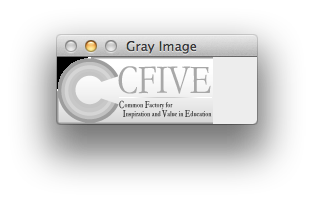
\includegraphics[width=5cm]{out_gray.png}

\includegraphics[width=5cm]{out_original.png}

\subsubsection{discussion}
このプログラムは引数として与えた画像ファイルを白黒に変換した画像ファイルを作成し、ウインドウを生成してオリジナル画像と白黒画像とを表示するプログラムである。  

6行めにあるようにOpenCVのプログラムでは名前空間としてcvというものがある。  

プログラムのmain関数内の10-13行目はコマンド引数が与えられなかったときにエラーメッセージを出力し、エラー終了するようになっている。  

このことは実行結果の引数を与えずに実行した場合に現れている。
\begin{quote}
\begin{verbatim}
grayscale  
usage: grascale <file>
\end{verbatim}
\end{quote}    
15行目でMat型変数imageに読み込んだ画像ファイルを代入している。  

OpenCVでは画像ファイルはMat型として扱われるが、これは画素値のrows\*cols行列である。  

16-19行目では画像ファイルの読み込みが成功したかどうかを確認している。  

Mat.dataメソッドは画素値を返すので、これに値が入っていかどうかで確認を行っている。  

21行目では生成する白黒画像を入れるためのMat型の変数grayImageを宣言している。  

22行目ではcvtColor関数を利用してimageの白黒画像をgrayImageに代入している。  

この関数は第一引数の画像データの色空間を変換し、その画像データを第二引数の変数に代入する。第三引数は色空間の変換指定で、CV\_BGR2GRAYはBGR色空間から白黒への変換を意味する。  

24,25行目では画像データの保存を行っている。関数imwriteは第一引数のファイルに第二引数の画像データを保存する。  

27-36行目はウインドウを生成し、オリジナルの画像と白黒変換後の画像を表示している。  

関数namedWindowは第一引数でウインドウの名前を指定しウインドウを生成する。第二引数はCV\_WINDOW\_AUTOSIZEのみが現在利用可能。  

関数imshowは第一引数に名前を与えられたウインドウに、第二引数に与えられた画像データを表示する。  

関数waitKeyは第一引数[ms]の間、キー入力を待ち、入力されたコードをかえす。引数に0を与えると無限に入力を待ち続ける。  

メソッドreleaseは画像データオブジェクトのデータを解放する。ここではwaitKey関数とあわせて利用され、キー入力によって画像表示を終える働きをしている。

\subsection{imageInfo.cc}
\subsubsection{source code}
\begin{verbatim}
     1	#include <iostream>
     2	#include <opencv2/core/core.hpp>              // OpevCVの基本機能(データ型)
     3	#include <opencv2/imgproc/imgproc.hpp>        // OpenCVで画像処理
     4	#include <opencv2/highgui/highgui.hpp>        // GUI のヘッダファイル
     5	
     6	using namespace cv;                           // OpenCV 名前空間
     7	using namespace std;
     8	
     9	int main(int argc, char* argv[]) {
    10	  if (argc <= 1) {                            // コマンド引数の説明
    11	    cerr << "usage: imageInfo <file>" << endl;
    12	    return -1;                                // エラー終了
    13	  }
    14	  Mat image = imread(argv[1]);                // 画像ファイルの読込み
    15	  if (!image.data) {                          // 読込みの成功確認
    16	    cerr << "no such file: " << argv[1] << endl;
    17	    return -1;                                // エラー終了
    18	  }
    19	  if (image.isContinuous())                   // データの連続性
    20	    cout << "isContinuous() = true" << endl;  // ギャップなし
    21	  else
    22	    cout << "isContinuous() = false" << endl; // ギャップあり
    23	  cout << "size of an element = " << image.elemSize() <<
    24	    " Bytes" << endl;                         // 1画素のバイト数
    25	  cout << "size of a channel  = " << image.elemSize1() <<
    26	    " Bytes" << endl;                         // 1channelのバイト数
    27	  cout << "type (hexadecimal) = " << hex << image.type() <<
    28	    dec << endl;                              // 画素のフォーマット
    29	  cout << "depth (hexadecimal) = " << hex << image.depth() <<
    30	    dec << endl;                              // 1channelのフォーマット
    31	  switch (image.depth()) {
    32	  case CV_8U:  cout << " CV_8U" << endl; break; // 8byte uchar
    33	  case CV_8S:  cout << " CV_8S" << endl; break; // 8byte char
    34	  case CV_16U: cout << " CV_16U" << endl; break;// 16byte ushort
    35	  case CV_16S: cout << " CV_16S" << endl; break;// 16byte short
    36	  case CV_32S: cout << " CV_32S" << endl; break;// 32byte int
    37	  case CV_32F: cout << " CV_32F" << endl; break;// 32byte float
    38	  case CV_64F: cout << " CV_64F" << endl; break;// 64byte double
    39	  defalut: cout << "    something else" << endl;// ありえない
    40	  }
    41	  cout << "size of a step    = " << image.step1() << endl;
    42	                  // 1行(row)のバイト数 = cols * elemSize() + ギャップ
    43	  cout << "no. of channels   = " << image.channels() << endl;
    44	                                              // 1画素のchannel数
    45	  cout << "no. of rows       = " << image.rows << endl;
    46	                                              // 画像の行数
    47	  cout << "no. of columns    = " << image.cols << endl;
    48	                                              // 画像の列数
    49	  namedWindow("Image", CV_WINDOW_AUTOSIZE);   // ウィンドウの生成
    50	  imshow("Image", image);                     // imageの表示
    51	  waitKey(0);                                 // キー入力待ち(無限)
    52	  image.release();                            // imageの解放
    53	
    54	  return 0;                                   // 正常終了
    55	}
\end{verbatim}

\subsubsection{result}
例題1と同じ画像ファイルlogo.pngを引数にあたえてimageInfoを実行した。  
\begin{quote}
imageInfo logo.png   
isContinuous() = true  
size of an element = 3 Bytes  
size of a channel  = 1 Bytes  
type (hexadecimal) = 10  
depth (hexadecimal) = 0  
 CV\_8U  
size of a step    = 468  
no. of channels   = 3  
no. of rows       = 67  
no. of columns    = 156  
\end{quote}

\includegraphics[width=5cm]{imageinfo.png}

\subsubsection{discussion}
このプログラムは引数に与えられた画像ファイルについての情報を出力するプログラムである。  

19行めのisContinuousメソッドは画像オブジェクトが連続的に要素を格納しているかどうかを返すメソッドである。  

すなわち、各行の最後にギャップが挿入されている場合はfalseを、そうでない場合はtrueを返す。  

23行目のelemSizeメソッドは1画素のバイト数を返す。この画像については3Bytesである。  

25行目のelemSize1メソッドは1チャネルのバイト数を返す。この画像については1Bytesである。  

27,29行目のtype,depthメソッドは画素,チャネルのフォーマットを返す。  

チャネルのフォーマットについては31\-40行で詳しく出力しており、この画像ではCV\_8Uすなわち8ビット符号なし整数である。  

以上をまとめるとこの画像ではRGB各色が0\-255の範囲で量子化されていることがわかった。  

41\-47行ではstep1,channels,rows,colsメソッドによって、それぞれステップ、チャネル、行、列の数が出力されている。

ステップ数とは一行のByte数で、この画像の場合各列が3Byteであること、列数が156列であること、行にギャップが挿入されていないことをあわせて、3\*156=468となっている。

\subsection{binary.cc}

\subsubsection{source code}
\begin{verbatim}
     1	#include<iostream>
     2	#include<opencv2/core/core.hpp>
     3	#include<opencv2/imgproc/imgproc.hpp>
     4	#include<opencv2/highgui/highgui.hpp>
     5	
     6	using namespace cv;
     7	using namespace std;
     8	
     9	#define TRACKBAR_MAX_VALUE   255
    10	#define THRESHOLD_MAX_VALUE  255
    11	
    12	const string windowName = "Binary";
    13	Mat grayImage; 
    14	void onChange(int value, void* data);
    15	
    16	int main(int argc, char* argv[]){
    17	  if (argc <= 1){
    18	    cerr << "usage: binary <file>" << endl;
    19	    return -1;
    20	  }
    21	
    22	  Mat image = imread(argv[1]);
    23	  if (!image.data){
    24	    cerr << "no such file: " << argv[1] << endl;
    25	    return -1 ;
    26	  }
    27	
    28	  cvtColor(image, grayImage, CV_BGR2GRAY);
    29	  image.release();
    30	  int value = 128;
    31	  namedWindow(windowName, CV_WINDOW_AUTOSIZE);
    32	  const string trackbarName = "Threshold";
    33	  createTrackbar(trackbarName, windowName, &value, TRACKBAR_MAX_VALUE,
    34			 onChange, NULL);
    35	  imshow(windowName, grayImage);
    36	  waitKey(0);
    37	  grayImage.release();
    38	
    39	  return 0;
    40	}
    41	
    42	void onChange(int value, void* data){
    43	  Mat binaryImage;
    44	  threshold(grayImage, binaryImage, value, THRESHOLD_MAX_VALUE,
    45		    THRESH_BINARY);
    46	  imshow(windowName, binaryImage);
    47	  binaryImage.release();
    48	}
\end{verbatim}

\subsubsection{result}
\begin{quote}
binary logo.png
\end{quote}

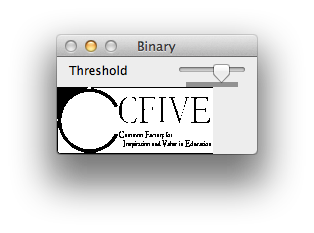
\includegraphics[width=5cm]{binary.png}

\subsubsection{discussion}
このプログラムはトラックバーのスライダを動かすことで、動的に画像の変換(この場合は)を行えるプログラムである。

createTrackbar関数は、第一引数を名前とするトラックバーを第二引数として与えられたウインドウ内に作成する。スライダの位置によって第三引数に与えた値が変化し、その最大値は第四引数に与えた値(このプログラムではTRACKBAR\_MAX\_VALUE)になる。スライダの位置が変更されると第五引数に与えられたコールバック関数が呼ばれる。第六引数はコールバック関数の台に引数に渡される。

threshold関数は、第一引数に与えられた画像データを第三引数を閾値として2値化して第二引数に書き出す。第五引数で二値化の種類を指定する。今の場合はTHRESH\_BINARYとなっていて、これは閾値を超えた値を第四引数の値(このプログラムではTHRESHOLD\_MAX\_VALUE)に書き換える。

このプログラムでは引数として与えた画像ファイルをimageに読み込み、cvtColorによってimageの白黒画像オブジェクトgrayImageを作っている。

その後、ウィンドウを生成し、トラックバーを生成し、grayImageを表示している。

ここでwaitKey関数により、キー入力待ちに入る。

そこでトラックバーを動かすと、コールバック関数onChangeが呼ばれる。

この関数の中では新しい画像データbinaryImageを作り、threshold関数によって、grayImageの値をvalue(128で初期化されていて、トラックバーの位置に応じて値がかわる。)を閾値として二値化してbinaryImageに書き出している。その後、imshow関数でウインドウにbinaryImageを表示している。

\subsection{レポート作成に要した時間}
2時間ほど
\subsection{特に苦労した点}
久しぶりにtexを書いた点。
\subsection{授業についての感想や希望}
特になし
\end{document}